\documentclass{article}
\usepackage{graphicx}
\usepackage{tikz}
\usetikzlibrary{arrows.meta, positioning}
\usepackage{hyperref}
\usepackage{geometry}
\geometry{margin=1in}
\title{RuralConnect Frontend Documentation}
\author{Your Team Name}
\date{\today}

\begin{document}
\maketitle

\tableofcontents
\newpage

% 1. Overview
\section{Overview}
\subsection{Project Purpose}
RuralConnect is a telemedicine platform designed to connect rural patients with healthcare professionals and services. The frontend is a React-based SPA that interacts with a Node.js/Express backend and a MongoDB database.

\subsection{Tech Stack}
\begin{itemize}
  \item \textbf{Frontend:} React, Vite, Tailwind CSS, Axios, Socket.io-client
  \item \textbf{Backend:} Node.js, Express, Socket.io, JWT, MongoDB (Mongoose)
  \item \textbf{Deployment:} GitHub Codespaces, Vercel/Netlify (frontend), Render/Heroku (backend)
\end{itemize}

\subsection{Architecture Diagram}
\begin{center}
  \includegraphics[width=0.8\textwidth]{architecture_diagram.png}
\end{center}

\subsection{Deployment Model}
The frontend is deployed as a static site (Vercel/Netlify), the backend as a Node.js server (Render/Heroku), and MongoDB is managed via Atlas. Environment variables are used for configuration.

% 2. Workflow and Page Linking
\section{Frontend Workflow and Page Linking}
\subsection{Page Navigation Diagram}
\begin{center}
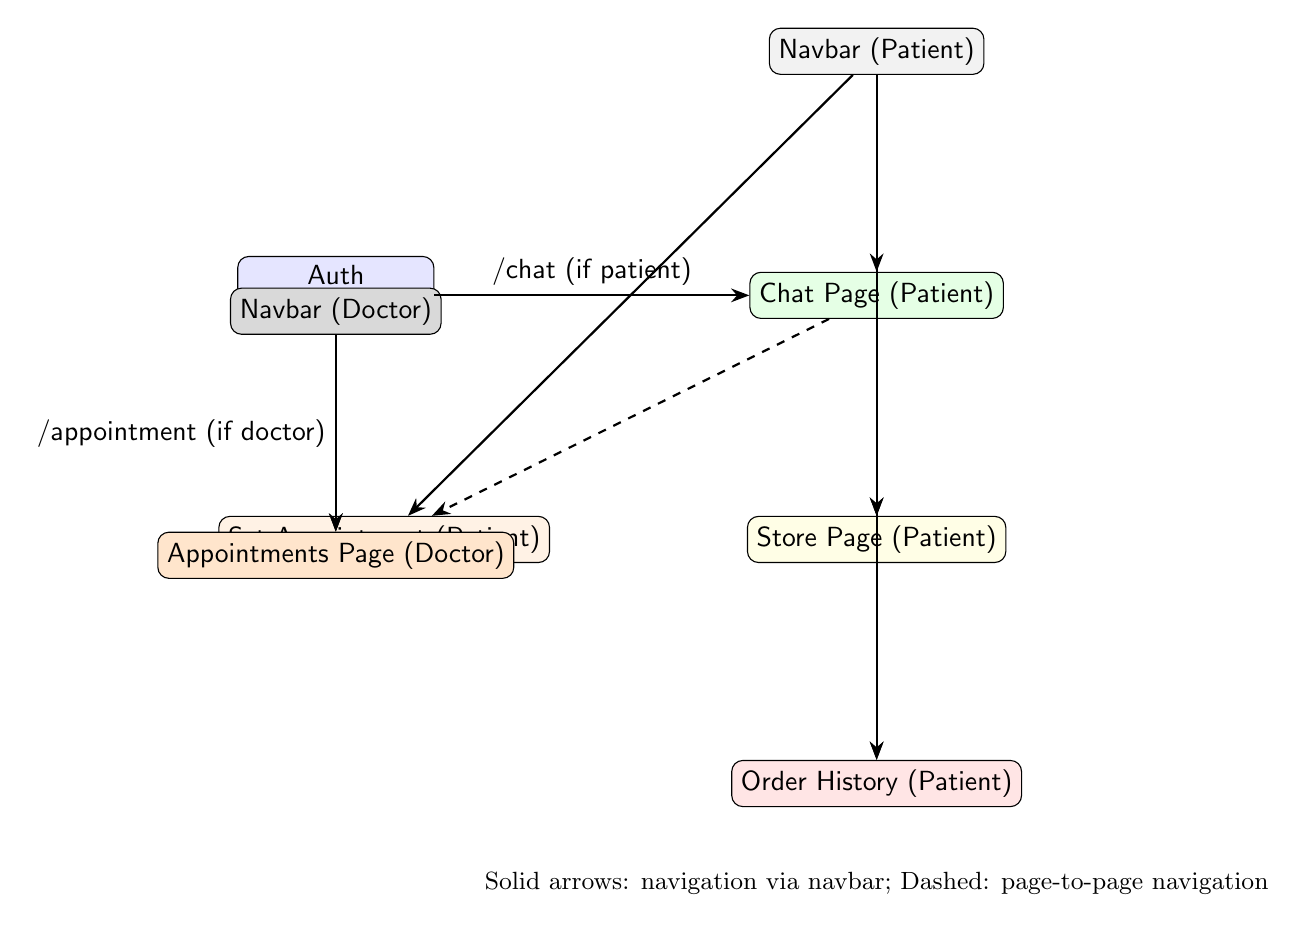
\begin{tikzpicture}[
  node distance=2.5cm,
  every node/.style={font=\sffamily, align=center},
  >=Stealth
]
% Nodes
\node[draw, rounded corners, fill=blue!10] (auth) {Auth\\(Login/Signup)};
% Patient flow
\node[draw, rounded corners, fill=green!10, right=4cm of auth] (chat) {Chat Page (Patient)};
\node[draw, rounded corners, fill=yellow!10, below=of chat] (store) {Store Page (Patient)};
\node[draw, rounded corners, fill=red!10, below=of store] (orderhistory) {Order History (Patient)};
\node[draw, rounded corners, fill=orange!10, left=of store] (setappt) {Set Appointment (Patient)};
% Doctor flow
\node[draw, rounded corners, fill=orange!20, below=of auth] (appointments) {Appointments Page (Doctor)};
% Navbars
\node[draw, rounded corners, fill=gray!10, above=of chat] (navbarp) {Navbar (Patient)};
\node[draw, rounded corners, fill=gray!30, above=of appointments] (navbard) {Navbar (Doctor)};

% Edges
% Auth to main pages
\draw[->, thick] (auth) -- node[above, sloped]{/chat (if patient)} (chat);
\draw[->, thick] (auth) -- node[left]{/appointment (if doctor)} (appointments);

% Patient navbar links
\draw[->, thick] (navbarp) -- (chat);
\draw[->, thick] (navbarp) -- (store);
\draw[->, thick] (navbarp) -- (orderhistory);
\draw[->, thick] (navbarp) -- (setappt);

% Patient page navigation
\draw[->, thick, dashed] (chat) -- (store);
\draw[->, thick, dashed] (store) -- (orderhistory);
\draw[->, thick, dashed] (chat) -- (setappt);

% Doctor navbar links
\draw[->, thick] (navbard) -- (appointments);

% Legends
\node[below=0.7cm of orderhistory, font=\small] {Solid arrows: navigation via navbar; Dashed: page-to-page navigation};
\end{tikzpicture}
\end{center}

\subsection{Page Descriptions}
\begin{itemize}
  \item \textbf{Auth:} Login/Signup, role selection (patient/doctor)
  \item \textbf{Chat:} Real-time chat with doctors, message history, new chat creation
  \item \textbf{Appointments:} View and manage appointments (doctor/patient views)
  \item \textbf{Store:} Browse and order medicines
  \item \textbf{Order History:} View past orders
  \item \textbf{Navbar:} Dynamic links based on user role
\end{itemize}

% 3. Getting Started
\section{Getting Started}
\subsection{Cloning the Repository}
\begin{verbatim}
git clone <repo-url>
cd RuralConnectFrontEnd
\end{verbatim}

\subsection{Environment Setup}
\begin{itemize}
  \item Node.js v18+
  \item npm v9+
  \item .env file with:
  \begin{verbatim}
VITE_BACKEND_URL=<backend-url>
  \end{verbatim}
\end{itemize}

\subsection{Installing Dependencies}
\begin{verbatim}
npm install
\end{verbatim}

\subsection{Running Locally}
\begin{verbatim}
npm run dev
\end{verbatim}

% 4. Authentication Flow
\section{Authentication}
\subsection{Login/Signup Flow}
\begin{enumerate}
  \item User submits login/signup form (role, email, password, etc.)
  \item Frontend sends POST to backend /api/users/login or /signup
  \item Backend validates, issues JWT (HttpOnly cookie)
  \item Frontend stores no token, relies on cookie for auth
  \item Protected routes checked via backend middleware
\end{enumerate}

\subsection{Token Structure and Expiration}
\begin{itemize}
  \item JWT contains user id, role, issued/expiry timestamps
  \item Expiration: 1h (configurable)
\end{itemize}

\subsection{Middleware Behavior}
\begin{itemize}
  \item Auth middleware checks JWT in cookies
  \item Sets req.user for downstream controllers
  \item Redirects/blocks on invalid/expired token
\end{itemize}

% 5. API Documentation
\section{API Documentation}
\subsection{Auth}
\begin{itemize}
  \item POST /api/users/login
  \item POST /api/users/signup
  \item GET /api/users/logout
  \item GET /api/users/me
\end{itemize}

\subsection{Chat}
\begin{itemize}
  \item POST /api/chat
  \item GET /api/chat/chatSummaries
  \item GET /api/chat/:chatId/messages
\end{itemize}

\subsection{Appointments}
\begin{itemize}
  \item GET /api/appointments
  \item POST /api/appointments
  \item etc.
\end{itemize}

\subsection{Store}
\begin{itemize}
  \item GET /api/medicine
  \item POST /api/order
  \item GET /api/order/history
\end{itemize}

\subsection{Error Format}
\begin{verbatim}
{
  success: false,
  message: "Error message",
  error: "Stack or details"
}
\end{verbatim}

% 6. Database Structures
\section{Database Structures}
\subsection{Schema Descriptions}
\begin{itemize}
  \item \textbf{User:} _id, name, email, password, role, chatIds, appointmentIds, etc.
  \item \textbf{Chat:} _id, title, lastMessage, messageHistory, participants
  \item \textbf{Message:} role, message, timestamp
  \item \textbf{Appointment:} _id, patientId, doctorId, time, status
  \item \textbf{Order:} _id, userId, items, status, timestamps
\end{itemize}

\subsection{Entity Relationships}
\begin{center}
  \includegraphics[width=0.8\textwidth]{erd.png}
\end{center}

\subsection{Data Validation}
\begin{itemize}
  \item All required fields validated in backend controllers
  \item Email/password format, role, etc. checked
\end{itemize}

% 7. Services and Modules
\section{Services and Modules}
\begin{itemize}
  \item \textbf{services/auth.js:} Handles login, signup, logout, profile fetch
  \item \textbf{services/chat.js:} Chat creation, summaries, messages
  \item \textbf{services/appointments.js:} Appointment CRUD
  \item \textbf{services/medicine.js:} Medicine and order APIs
  \item \textbf{components/Chat/:} Chat UI components
  \item \textbf{pages/:} Page-level components for routing
\end{itemize}

% 8. Error Handling and Logging
\section{Error Handling and Logging}
\begin{itemize}
  \item All API errors return a standard format (see above)
  \item Frontend displays error messages via alerts or UI banners
  \item Backend logs errors to console and optionally to a file/service
\end{itemize}

\section{Diagrams}
\textbf{Note:} Replace the placeholders (architecture\_diagram.png, frontend\_workflow.png, erd.png) with your actual diagrams.

\end{document}
